\documentclass[11pt,a4paper]{report}
\usepackage[margin=1in]{geometry}
\usepackage{times}
\usepackage{setspace}
\usepackage{booktabs}
\usepackage{longtable}
\usepackage{array}
\usepackage{tabularx}
\usepackage{enumitem}
\usepackage{graphicx}
\usepackage{xcolor}
\usepackage{fancyhdr}
\usepackage{titlesec}
\usepackage{hyperref}
\usepackage[T1]{fontenc}
\usepackage[utf8]{inputenc}

\hypersetup{
  colorlinks=true,
  linkcolor=blue!50!black,
  urlcolor=blue!50!black,
  citecolor=blue!50!black,
  pdftitle={AMPscan: Binary Antimicrobial Peptide Classifier},
  pdfauthor={NIT Raipur SIH-style team}
}
\onehalfspacing
\setlength{\parskip}{0.35em}
\setlist[itemize]{leftmargin=1.4em,itemsep=0.2em}
\setlist[enumerate]{leftmargin=1.6em,itemsep=0.25em}
\pagestyle{fancy}
\fancyhf{}
\fancyhead[L]{\small AMPscan study guide}
\fancyhead[R]{\small NIT Raipur SIH-style}
\fancyfoot[C]{\thepage}
\renewcommand{\headrulewidth}{0.4pt}

\newcommand{\RF}{0.9515}
\newcommand{\RFrand}{0.9791}

\title{\textbf{AMPscan: Binary Antimicrobial Peptide Classifier}\\[0.6em]
\large Complete Team Study Guide\\
(Internal NIT Raipur SIH-style hackathon)}
\author{B.Tech.\ Biotechnology (5th semester)\\
Student laptop --- NVIDIA GeForce RTX 5060 Laptop GPU (8\,GB VRAM), 16\,GB RAM\\
Offline demo; no paid APIs}
\date{Locked snapshot: Phases 1--9}

\begin{document}
\maketitle
\begin{abstract}
\textbf{AMPscan} is a homology-aware binary classifier for short peptides (length 5--100 amino acids): antimicrobial peptide (AMP) versus non-AMP. It was built as a \emph{scoped} answer to the official SIH problem ``AI-Based Protein and Biomolecule Classification Assistant.'' Positives come from DRAMP General (CC BY~4.0); negatives from published AMPlify non-AMP FASTA files (Zenodo 10.5281/zenodo.7320306, CC BY~4.0). Sequences are clustered with MMseqs2 at 30\% identity (coverage 0.8, cov-mode~1); whole clusters go to train, validation, or test so close homologs do not leak across folds. On that hard split a Random Forest on composition features reaches homology-test ROC-AUC~\textbf{0.9515} (accuracy 0.8734). Frozen ESM-2 35M and a 1D-CNN sit slightly below; frozen ESM-2 150M is a \textbf{tie} at 0.9521. Random-split RF ROC-AUC 0.9791 is shown only as a leakage control. The Streamlit demo reports Platt-calibrated RF as the primary score. Magainin-2, LL-37, and melittin are \textbf{in the training set}. This is a sequence-pattern filter, not a wet-lab assay.
\end{abstract}
\tableofcontents
\clearpage

\chapter{Official problem versus our scope}
\label{ch:scope}

\section{Two titles}

\begin{tabularx}{\textwidth}{>{\bfseries}l X}
Official SIH title & AI-Based Protein and Biomolecule Classification Assistant \\
Our scoped title & \textbf{AMPscan: Binary Antimicrobial Peptide Classifier} \\
\end{tabularx}

The official brief asks for FASTA in, reproducible preprocessing, classification into functional or biological categories, confidence scores, and some form of explainability. That wording could mean Gene Ontology (GO) for all proteins, Pfam domains, enzyme classes, subcellular location, or peptides. We chose \textbf{one} axis we could finish honestly on a student laptop.

\section{Why not all proteins, GO, or Pfam}

GO has thousands of terms, hierarchical metrics, and extreme class imbalance. Pfam, done properly, is a sequence-search database (HMMER), not a 3-day neural net. Full-length proteins on an 8\,GB GPU cannot be fine-tuned at foundation-model scale in a hackathon. A wide GO/Pfam demo with a \emph{random} train/test split will look excellent and still leak homology. AMPscan instead finishes AMP versus non-AMP with a \textbf{cluster split}, calibration, and residue plots.

\section{What success means here}

Success is: a working offline FASTA demo; locked homology-test numbers you can defend; a clear story about leakage; and the sentence ``this is not a killing assay.'' Success is \emph{not} claiming Nature-level AMP discovery or a universal protein classifier.

\chapter{Biological background}
\label{ch:bio}

\section{What antimicrobial peptides are}

An \textbf{antimicrobial peptide (AMP)} is a short chain of amino acids that can damage microbes, often by disrupting membranes. In this project ``AMP'' means \emph{labelled AMP in DRAMP General}, not ``we measured a minimum inhibitory concentration.''

\section{Why classify AMP versus non-AMP}

Public AMP databases exist; people train models to flag new sequences that \emph{look like} known AMPs. That can triage candidates before synthesis. The scientific risk is treating a database look-alike score as experimental activity.

\section{Length 5--100}

AMPs used in prediction papers are typically short. We locked \textbf{5 to 100} amino acids inclusive. AMPlify originally allowed up to 200; we tightened the window. Longer proteins are out of spec: the app rejects them. Short length is also why \textbf{composition} (how many lysines, how hydrophobic) is so informative.

\section{Natural versus synthetic AMPs}

DRAMP General mixes peptides isolated from nature and peptides that were \textbf{synthesized} in a lab, often designed to look amphipathic and cationic. Composition models (our Random Forest) are helped by those designs. Performance on a purely natural, phylogenetically new set was \emph{not} measured.

\chapter{End-to-end pipeline}
\label{ch:pipe}

\begin{verbatim}
DRAMP General FASTA          AMPlify non-AMP FASTAs
        \                          /
         -> length 5-100, alphabet, dedup
                    |
         combined_clean.fasta (21,337)
                    |
         MMseqs2 easy-cluster 30% / 0.8 / cov-mode 1
                    |
         whole clusters -> train / val / test  (70/15/15)
                    |
    +---------------+---------------+
    |               |               |
   RF+logreg     frozen ESM      1D-CNN
   (composition)  35M & 150M     one-hot
    |               |               |
    Platt          T scaling       T scaling
    |               |               |
    Streamlit: primary = calibrated RF
               secondary = T-scaled CNN
               IG heatmap (CNN); train-set banner
\end{verbatim}

Locked roots: \texttt{data/} (raw, processed, splits), \texttt{models/} (baseline, esm2\_35M, esm2\_150M, cnn1d, calibration), \texttt{reports/}, \texttt{app/streamlit\_app.py}. Do not retrain for the pitch.

\chapter{Data}
\label{ch:data}

\section{Sources and licenses}

\begin{tabular}{llp{0.42\textwidth}}
\toprule
Role & Source & License / cite \\
\midrule
Positives & DRAMP General FASTA & CC BY 4.0; Ma et al.\ NAR 2025; Shi et al.\ NAR 2022 \\
Negatives & AMPlify non-AMP FASTAs, DOI 10.5281/zenodo.7320306 & CC BY 4.0; Li et al.\ BMC Genomics 2022; BMC Res Notes 2023 \\
\bottomrule
\end{tabular}

Raw DRAMP General: \textbf{11{,}687} records. APD and UniProt Swiss-Prot were listed as fallbacks and were \textbf{not} used.

\section{Why AMPlify negatives}

``Non-AMP'' is not a natural biological class. AMPlify already published FASTA negatives for this ML setting. That is more documentable than an ad hoc UniProt keyword scrape. We used their \textbf{balanced} train+test files first. After cleaning, unique negatives were still fewer than unique AMPs, so we added \textbf{6{,}579} sequences from the published \textbf{imbalanced} AMPlify non-AMP files---not a new Swiss-Prot sample.

\section{Cleaning rules}

\begin{enumerate}
\item Length 5--100 inclusive.
\item Uppercase. Map B, Z, U, O, J $\rightarrow$ X. Drop leftover non-amino-acid characters. \textbf{X is allowed.}
\item Exact-sequence deduplication; keep first occurrence.
\item Same sequence labelled both AMP and non-AMP: \textbf{keep AMP} (19 conflicts).
\end{enumerate}

Mapped B/Z/U/O/J$\rightarrow$X: 418 positives, 0 negatives. Dropped leftover non-AA: 48 positives, 0 negatives.

\section{Cleaning funnel (locked)}

\begin{tabular}{lrr}
\toprule
Stage & AMP & non-AMP \\
\midrule
Raw (DRAMP / AMPlify balanced) & 11687 & 4173 \\
Length 5--100 & 11459 & 4099 \\
After alphabet & 11411 & 4099 \\
After exact dedup & 10678 & 4099 \\
$+$ imbalanced AMPlify & --- & $+$6579 \\
After conflict resolve & \textbf{10678} & \textbf{10659} \\
\bottomrule
\end{tabular}

Combined clean set: \textbf{21{,}337} peptides.

\section{What we do not claim about labels}

Negatives mean ``not annotated as AMP in that construction,'' not ``experimentally inactive.'' Some AMPs are synthetic or weak. DRAMP General is not a MIC table. A later audit of the DRAMP \texttt{Family} column found \textbf{4{,}841} cleaned AMPs with a family string and \textbf{5{,}837} missing; the column mixes peptide families with virus taxa. \textbf{No family-class head was trained.}

\chapter{Homology and MMseqs2}
\label{ch:homology}

This chapter is the one you must be able to speak without notes.

\section{Homology and sequence identity}

\textbf{Homology} here means ``these sequences look related'': they share enough amino acids in an alignment. \textbf{Sequence identity} is the fraction of aligned positions that match. If identity is high, a model can memorize the family instead of learning a general AMP pattern.

\section{Why random train/test splits leak}

If you shuffle peptides into train and test, a test peptide can be a near-copy of a training peptide. Accuracy of 0.98 then means ``I have seen your cousins,'' not ``I understand AMPs.'' That is \textbf{homology leakage}.

\section{What MMseqs2 \texttt{easy-cluster} does}

MMseqs2 is a fast clustering tool. \texttt{easy-cluster} puts similar sequences in the same \textbf{cluster} (think: household of relatives). We clustered the \emph{combined} AMP$+$non-AMP set so a similar AMP and non-AMP cannot land in different folds.

\section{The three flags}

\begin{description}[style=nextline]
\item[\texttt{-\/-min-seq-id 0.3}] Cluster together if identity is about \textbf{30\%} or more. Stricter than the 70--90\% cuts some papers use.
\item[\texttt{-c 0.8}] Require \textbf{80\% coverage} of the relevant sequence by the alignment.
\item[\texttt{-\/-cov-mode 1}] Coverage applies to the \textbf{shorter} sequence. Fair when a 20-aa AMP is compared to a 90-aa fragment: the short one must be mostly covered.
\end{description}

\section{Whole-cluster assignment}

Every member of a cluster goes to \textbf{one} fold: train, validation, or test. Targets $\approx$ 70/15/15 of sequences, seed 42. Clusters were stratified as AMP-only, non-AMP-only, or mixed so neither class vanishes from a fold.

\textbf{9{,}241 clusters:} 4{,}778 AMP-only, 4{,}391 non-AMP-only, \textbf{72 mixed}.

\begin{tabular}{lrrr}
\toprule
Fold & $n$ & AMP & non-AMP \\
\midrule
Train & 14904 & 7444 & 7460 \\
Val & 3203 & 1611 & 1592 \\
Test & 3230 & 1623 & 1607 \\
\bottomrule
\end{tabular}

\section{Mixed clusters}

Seventy-two clusters contain \emph{both} an AMP and a non-AMP (264 AMP members, 445 non-AMP). They still stay in \textbf{one} fold---so they do not leak across train/test. They \emph{do} show that 30\% identity is not a biological force field: a short AMP can sit inside a longer UniProt-like peptide. Mixed-cluster AMPs are shorter on average (mean 46.6\,aa) than mixed-cluster non-AMPs (mean 62.9\,aa). Full table: \texttt{reports/mixed\_clusters.md}.

\section{Leakage-gap numbers}

\begin{tabular}{lcc}
\toprule
Model & Homology test ROC-AUC & Random-split test ROC-AUC \\
\midrule
Random Forest & \textbf{0.9515} & 0.9791 \\
ESM-2 35M linear (frozen) & 0.9450 & 0.9657 \\
1D-CNN & 0.9424 & 0.9749 \\
ESM-2 150M linear (frozen) & 0.9521 & (not used as the test comparison) \\
\bottomrule
\end{tabular}

The extra points on the random split are leakage. Quote \textbf{0.95}.

\section{30-second judge version}

``We clustered peptides at 30\% identity with MMseqs2, coverage 80\% on the shorter sequence, and never split a cluster across train and test. Random-split RF ROC-AUC is 0.98; homology-split is 0.95. We report 0.95. The gap is leakage, not better biology.''

\chapter{Features and classical model}
\label{ch:rf}

\section{What the forest sees}

425 numbers per peptide:
\begin{itemize}
\item \textbf{AAC} (20): fraction of each standard amino acid.
\item \textbf{DPC} (400): fraction of each adjacent pair (20$\times$20).
\item \textbf{Length}.
\item \textbf{Net charge at pH~7}: Henderson--Hasselbalch, including N- and C-termini.
\item \textbf{GRAVY}: mean Kyte--Doolittle hydrophobicity.
\item \textbf{Hydrophobic moment}: Eisenberg scale, $100^\circ$ per residue (helix assumption), divided by length.
\item \textbf{Aromatic fraction}: (F$+$W$+$Y)/length.
\end{itemize}

X is ignored in AAC/DPC counts but still counted in length.

\section{Why composition is strong here}

AMPs in databases are often short, cationic, and amphipathic. Frequency of K/R, hydrophobics, and net charge already separate them from typical UniProt fragments of similar length. That is why a forest can match a protein language model.

\section{Locked homology-test metrics}

\begin{tabular}{lcccc}
\toprule
Model & Acc. & Macro-F1 & ROC-AUC & PR-AUC \\
\midrule
\textbf{Random Forest (primary)} & \textbf{0.8734} & \textbf{0.8734} & \textbf{0.9515} & \textbf{0.9542} \\
Logistic regression (L2) & 0.8375 & 0.8374 & 0.9016 & 0.9113 \\
\bottomrule
\end{tabular}

RF confusion on homology test ($n=3230$): TN 1388, FP 219, FN 190, TP 1433. Class weight balanced; 200 trees; seed 42. The Streamlit \textbf{primary} score is this RF after Platt calibration.

\chapter{Deep learning models}
\label{ch:dl}

No ESM weights were updated (frozen encoder). The 1D-CNN was trained from scratch on one-hot sequences, \emph{not} on ESM embeddings.

\section{Locked homology-test comparison}

\begin{tabular}{lcccc}
\toprule
Model & Acc. & Macro-F1 & ROC-AUC & PR-AUC \\
\midrule
RF (Phase 2) & 0.8734 & 0.8734 & \textbf{0.9515} & 0.9542 \\
ESM-2 35M linear, frozen (Phase 3) & 0.8622 & 0.8622 & 0.9450 & 0.9424 \\
1D-CNN (Phase 4) & 0.8650 & 0.8648 & 0.9424 & 0.9465 \\
ESM-2 150M linear, frozen (Phase 9) & 0.8762 & 0.8761 & 0.9521 & 0.9516 \\
\bottomrule
\end{tabular}

Phase 9 versus RF: $\Delta$ ROC-AUC \textbf{$+$0.0006} on test --- a \textbf{tie}. Phase 9 \textbf{validation} ROC-AUC was \textbf{0.9372}, so LoRA was \textbf{not} run (protocol required val within 0.01 of RF).

\section{Architectures in one paragraph each}

\textbf{ESM-2 35M} (\texttt{facebook/esm2\_t12\_35M\_UR50D}): 12 layers, hidden size 480. Mean-pool residue tokens; drop CLS/EOS/PAD. Linear (logistic) head, class-balanced, features StandardScaled on train.

\textbf{1D-CNN}: 21 input channels (20 amino acids $+$ X), length padded to 100 with zeros. Convolutions 21$\rightarrow$64 ($k=5$), 64$\rightarrow$128 ($k=5$), 128$\rightarrow$128 ($k=3$), global max pool, dense 128$\rightarrow$64$\rightarrow$1. Dropout 0.20 selected on val. $\sim$105k parameters.

\textbf{ESM-2 150M} (\texttt{facebook/esm2\_t30\_150M\_UR50D}): 30 layers, hidden 640. Same frozen mean-pool recipe. Linear head. Homology test scored \textbf{once} after val selection.

\section{Frozen versus fine-tune versus LoRA}

\begin{description}
\item[Frozen] Encoder weights never change; only a small head is fit. What we did.
\item[Fine-tune] Update (almost) all encoder weights. Too heavy and leak-prone for this laptop/task.
\item[LoRA] Low-rank adapters: a cheap partial fine-tune. \textbf{Not trained.} Val was not within 0.01 ROC-AUC of RF.
\end{description}

\section{Why frozen protein LMs did not clearly beat RF}

ESM is trained on long evolutionary proteins. Our peptides are short; the label is largely composition. Frozen 35M \emph{lost}; frozen 150M \emph{tied}. That is a scientific result: on this split you do not need a 150M encoder to ship a demo.

\chapter{Calibration}
\label{ch:cal}

\section{Confidence is not accuracy}

ROC-AUC asks whether AMPs get \emph{higher scores} than non-AMPs. A model can rank perfectly and still say ``99\% AMP'' when it is wrong half the time in that bin. \textbf{Calibration} adjusts probabilities so that ``80\%'' happens about 80\% of the time.

\section{Two methods (do not mix the names)}

\begin{itemize}
\item \textbf{Temperature scaling} (ESM-2 35M and CNN): $p=\mathrm{sigmoid}(\mathrm{logit}/T)$, $T>0$ fit by negative log-likelihood on \textbf{homology val}. $T>1$ cools over-confident logits. CNN $T=1.2833$ (app uses 1.283). ESM-2 35M $T=1.2855$.
\item \textbf{Platt scaling} (RF only): $p=\mathrm{sigmoid}(a\cdot p_{\mathrm{RF}}+b)$ with $a=10.0847$, $b=-5.0839$, fit on homology val RF probabilities. \textbf{This is not temperature scaling.}
\end{itemize}

\section{ECE and Brier}

\textbf{ECE} (15 equal-width bins on $[0,1]$): average $|$predicted probability $-$ empirical AMP rate$|$, weighted by bin count. Lower is better. \textbf{Brier}: mean squared error of $P(\mathrm{AMP})$ versus 0/1.

\section{Locked homology-test calibration}

\begin{tabular}{lcccc}
\toprule
Model & Uncal ECE & Cal ECE & Uncal Brier & Cal Brier \\
\midrule
RF (Platt) & 0.0776 & \textbf{0.0235} & 0.0958 & 0.0883 \\
ESM-2 35M (T) & 0.0376 & \textbf{0.0185} & 0.0956 & 0.0938 \\
1D-CNN (T) & 0.0624 & \textbf{0.0403} & 0.0991 & 0.0957 \\
\bottomrule
\end{tabular}

ROC-AUC is \textbf{unchanged} (0.9515 / 0.9450 / 0.9424): $T$ and Platt with $a>0$ are monotone, so ranking is preserved.

\chapter{Explainability}
\label{ch:xai}

\section{Integrated Gradients and occlusion}

Only the \textbf{1D-CNN} was attributed. \textbf{Integrated Gradients} (Captum) on the 21-channel one-hot, baseline all zeros, target $=$ AMP logit. Per-residue score $=$ sum of attributions over 21 channels at that position. \textbf{Occlusion}: set one residue's column to zero; $\Delta=$ logit$_{\mathrm{full}}-$ logit$_{\mathrm{occluded}}$.

\section{What a heatmap means and does not mean}

Red / positive IG: that position \emph{as encoded} pushes the CNN AMP logit up. It is \textbf{not} a binding site, not mutagenesis data, not a mechanism.

\section{Canonical peptides --- they are in train}

\begin{tabular}{lll}
\toprule
Peptide & Sequence & Homology train ID \\
\midrule
magainin-2 & GIGKFLHSAKKFGKAFVGEIMNS & POS\_DRAMP\_DRAMP02271 \\
LL-37 & LLGDFFRKSKEKIGKEFKRIVQRIKDFLRNLVPRTES & POS\_DRAMP\_DRAMP03571 \\
melittin & GIGAVLKVLTTGLPALISWIKRKRQQ & POS\_DRAMP\_DRAMP03002 \\
\bottomrule
\end{tabular}

None are in val or test. \textbf{Say this every time you show them:} ``These three examples are in the training set.'' That is the opposite of fake held-out validation.

High $|$IG$|$ often lands on K/R (cationic) or hydrophobic/aromatic residues---consistent with the textbook AMP cartoon. Pearson IG versus occlusion: magainin-2 0.89, LL-37 0.35, melittin 0.91. Correlation, not causation.

If the figures below render, they are the locked Phase-6 heatmaps.

\begin{center}
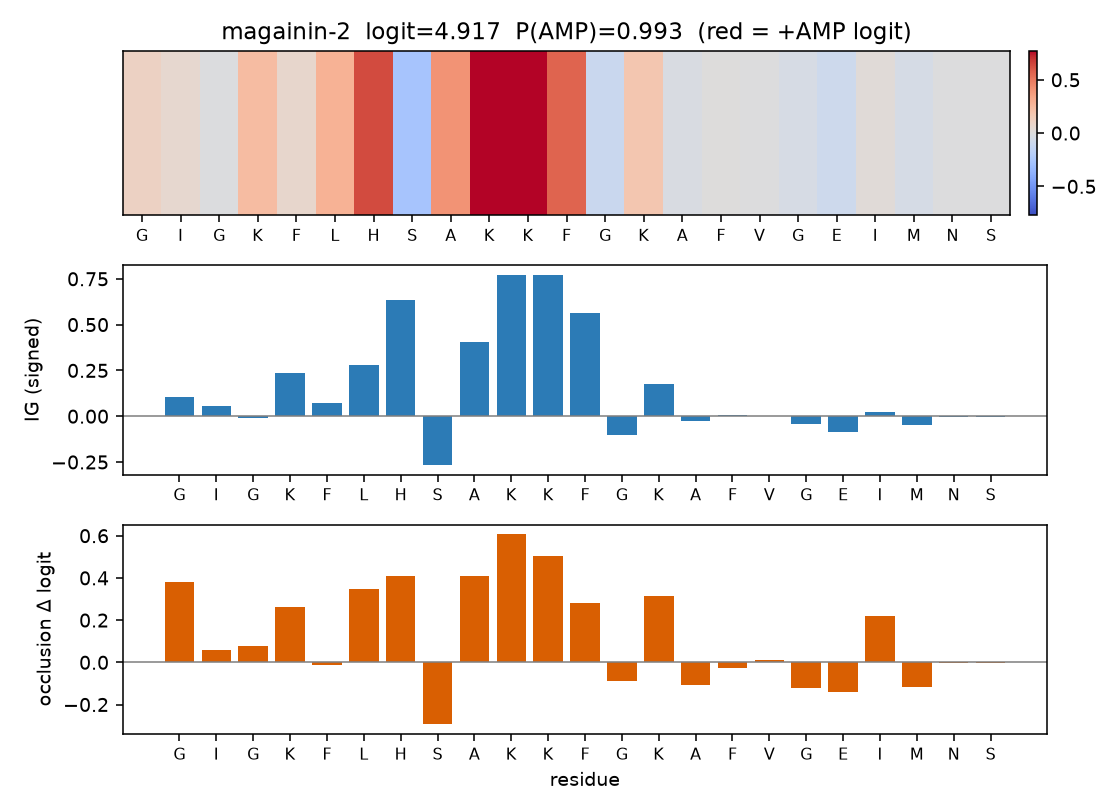
\includegraphics[width=0.95\textwidth]{../explain/heatmap_magainin_2.png}\\[0.4em]
{\small Magainin-2 (training example).}
\end{center}

\chapter{Demo}
\label{ch:demo}

\section{How to run}

From the project root, conda env \texttt{amp-data}:
\begin{verbatim}
streamlit run app/streamlit_app.py
\end{verbatim}
Open the printed localhost URL (typically \texttt{http://localhost:8501}).

\section{What the scores are}

\begin{itemize}
\item \textbf{Primary:} Platt-calibrated Random Forest $P(\mathrm{AMP})$. Label AMP / non-AMP at 0.5 on this score.
\item \textbf{Secondary:} CNN $P(\mathrm{AMP})$ after temperature $T=1.283$.
\item Also shown: length, net charge at pH~7, GRAVY.
\end{itemize}

Invalid sequences (length outside 5--100, leftover non-AA after B/Z/U/O/J$\rightarrow$X) error out. FASTA upload is capped at 50 sequences. ESM-150M is \textbf{not} loaded in the app (too heavy); it appears only as a locked number on Metrics.

\section{Metrics page}

Homology table (RF 0.9515, 35M 0.9450, CNN 0.9424, 150M 0.9521 tie); random-split leakage table; ECE before/after; limitations paragraph.

\section{90-second spoken script}

``Official SIH title is an AI protein classifier. We scoped it to AMPscan: AMP versus not, length 5 to 100, because we could finish that honestly on an 8\,GB laptop. The silent bug is homology leakage. We clustered at 30\% identity and kept whole clusters in one fold. 21{,}337 peptides, about 10.7k AMPs from DRAMP, 10.7k non-AMPs from AMPlify. On that hard split a random forest on composition gets ROC-AUC 0.95. Frozen ESM-2 35M is 0.945. CNN 0.942. Frozen 150M is 0.952---a tie. Random-split RF is 0.98; that extra is leakage. The demo's main number is Platt-calibrated RF. Magainin-2 is in training. This is not a wet-lab AMP test.''

\section{4-minute spoken script}

Add: cleaning rules and 19 conflicts kept as AMP; extra AMPlify imbalanced negatives; RF ECE 0.078 to 0.023; live paste of magainin plus the banner; Metrics homology versus random; ``GO/Pfam is a different problem and usually no cluster split''; close with ``one functional axis, leak controlled, confidence calibrated.''

\chapter{Limitations}
\label{ch:lim}

\begin{enumerate}
\item Sequence-pattern classifier, not a measurement of killing.
\item Test is $\approx$50/50. Real proteomes are AMP-rare; precision would collapse unless the threshold rises.
\item Negatives are unannotated, not proven inactive.
\item DRAMP General includes synthetics that help composition models.
\item 72 mixed clusters: 30\% identity is strict, not perfect.
\item Random-split 0.98 is leaky; quote 0.95.
\item Frozen ESM and CNN did not clearly beat RF. Composition carries most of the short-peptide signal.
\item IG is not mechanism. Famous AMPs are in \textbf{train}.
\item Out of scope: full proteins, GO, Pfam, EC, MIC, hemolysis, in vivo.
\end{enumerate}

The official title is broader than the deliverable. That is intentional scoping, not unfinished work.

\chapter{Rejections and laptop limits}
\label{ch:reject}

\section{What we refused and why}

\begin{description}
\item[GO / all-UniProt function] Thousands of labels, hierarchical metrics, needs a different split. 8\,GB will not fine-tune a proteome-scale GO model this week.
\item[Pfam as ``our neural net''] Real Pfam is HMMER. A two-day classifier on Pfam-A almost certainly leaks homology.
\item[ESM 3B/15B] Does not fit this GPU for serious work; frozen 150M already tied RF.
\item[DeepLoc] Different task (subcellular location of proteins), different data.
\item[Family 5--10 class head] DRAMP \texttt{Family} is 55\% missing on our AMPs and mixes virus taxa with peptide families. Cyclotide has 1 homology-test sequence. Audit: no-go. \texttt{reports/family\_label\_audit.md}.
\end{description}

\section{If another team demos GO/Pfam}

Ask which identity split they used. If they cannot name CD-HIT or MMseqs, their F1 is not comparable. If Pfam is HMMER, that is a database hit. We refuse length $>$100 rather than invent GO terms at 0.99 confidence.

\chapter{Glossary}
\label{ch:gloss}

\begin{description}[style=nextline,leftmargin=0pt,font=\bfseries]
\item[AAC] Amino-acid composition: 20 frequencies.
\item[Accuracy] Fraction correct at threshold 0.5; here $\approx$0.87 on a balanced test.
\item[AMP] Antimicrobial peptide; in this repo, a DRAMP General label.
\item[AMPlify] Published AMP predictor and FASTA sets used for negatives.
\item[AMPscan] This project: binary homology-aware AMP classifier.
\item[Brier score] Mean squared error of predicted $P(\mathrm{AMP})$.
\item[CC BY 4.0] Cite the source; reuse allowed.
\item[Cluster] MMseqs2 group of similar sequences; assigned wholly to one fold.
\item[CNN] Convolutional neural net; here 1D over one-hot peptides.
\item[Coverage] How much of a sequence is in the alignment (80\%, shorter seq).
\item[DRAMP] Data Repository of Antimicrobial Peptides; our positive source.
\item[DPC] Dipeptide composition: 400 pair frequencies.
\item[ECE] Expected Calibration Error; 15 bins in our tables.
\item[ESM-2] Evolutionary Scale Modeling protein language model (Meta).
\item[FASTA] Text format: \texttt{>} header then sequence letters.
\item[Frozen] Encoder weights not updated.
\item[GO] Gene Ontology; not this project.
\item[GRAVY] Average Kyte--Doolittle hydrophobicity.
\item[Homology] Sequence-similarity relatedness (as used here).
\item[Homology split] Whole clusters to train/val/test; our honest split.
\item[Hydrophobic moment] Helix amphipathicity score (Eisenberg, $100^\circ$/res).
\item[IG] Integrated Gradients; attribution on CNN one-hot.
\item[Identity] Fraction of aligned residues that match (we used 30\%).
\item[Leakage] Train/test sharing close homologs; inflates metrics.
\item[Logit] Raw score before sigmoid.
\item[LoRA] Cheap fine-tune method; \textbf{not run}.
\item[Macro-F1] F1 averaged over AMP and non-AMP.
\item[Mean-pool] Average of residue embeddings, skipping special tokens.
\item[MIC] Minimum inhibitory concentration; not predicted here.
\item[Mixed cluster] Cluster containing both AMP and non-AMP (72 of them).
\item[MMseqs2] Fast sequence clustering/search tool.
\item[Net charge] Approximate charge at pH~7 including termini.
\item[Occlusion] Hide one residue; measure logit change.
\item[One-hot] 21-channel switch vector per position (20 AA $+$ X).
\item[Pfam] Protein domain database; not this project.
\item[Platt scaling] Logistic map on RF probabilities.
\item[PR-AUC] Area under precision--recall curve.
\item[Random Forest] Ensemble of decision trees; our primary model.
\item[Random split] Shuffle ignoring clusters; leaky control.
\item[ROC-AUC] Ranking quality; 0.5 chance, 1 perfect order. Not ``percent correct.''
\item[Seed 42] Fixed random seed for splits and models.
\item[Temperature scaling] Divide logits by $T$; used for CNN and ESM-35M.
\item[Val / test] Validation for choices; test scored sparingly (150M: once).
\item[VRAM] GPU memory; this laptop has 8\,GB.
\end{description}

\chapter{Judge Q\&A}
\label{ch:qa}

Answers are 20--40 seconds. Use these numbers.

\begin{enumerate}[leftmargin=1.6em]
\item \textbf{What do you predict?} $P(\mathrm{AMP})$ for a 5--100\,aa peptide under a 30\% cluster split. Not MIC.

\item \textbf{Why not all proteins?} Finishability, 8\,GB VRAM, and a split we can defend. GO is another project.

\item \textbf{What is homology leakage?} Cousins in train and test. The model memorizes the family.

\item \textbf{What did MMseqs2 do?} Cluster at 30\% identity, 80\% coverage on the shorter sequence; whole cluster to one fold.

\item \textbf{Why 30\% not 90\%?} Stricter. Harder, more honest.

\item \textbf{What is cov-mode 1?} Coverage of the \emph{shorter} sequence.

\item \textbf{Random AUC is higher---why report 0.95?} Random RF 0.979 is leaky. Homology RF 0.9515 is the claim.

\item \textbf{Why is RF primary if you have ESM?} RF 0.9515; 35M 0.945; 150M 0.9521 tie. RF is CPU-fast and calibrated.

\item \textbf{Did 150M beat RF?} By $+$0.0006. Tie. Val 0.937 so no LoRA.

\item \textbf{Why not fine-tune?} VRAM, and frozen already ties composition RF.

\item \textbf{Where are negatives from?} AMPlify published non-AMP FASTAs, CC BY 4.0. Then extra from their imbalanced files.

\item \textbf{Are labels perfect?} No. Non-AMP $\neq$ inactive. 19 conflicts kept as AMP.

\item \textbf{Platt or temperature on RF?} Platt. $a=10.08$, $b=-5.08$. Do not say temperature.

\item \textbf{CNN $T$?} $T=1.283$. Cools overconfidence. ROC-AUC unchanged.

\item \textbf{What is ECE?} Calibration error, 15 bins. RF 0.078 $\rightarrow$ 0.023 after Platt.

\item \textbf{Can I trust 0.99 on a proteome?} No. Test is 50/50; nature is not.

\item \textbf{What does the heatmap mean?} CNN IG on residues. Not a binding site. Magainin-2 is in \textbf{train}.

\item \textbf{Did you test famous AMPs as held-out?} No. Magainin-2, LL-37, melittin are train IDs DRAMP02271, 03571, 03002.

\item \textbf{72 mixed clusters---is that leakage?} Not across folds. It means some AMP/non-AMP pairs are still 30\%-similar.

\item \textbf{Why 5--100?} Peptide AMP range we locked. Longer sequences are rejected.

\item \textbf{Natural or synthetic?} DRAMP General is both. That helps composition models.

\item \textbf{Did you beat AMPlify the paper?} Different data and split. We do not claim their AUC.

\item \textbf{Family classification?} Audited: 55\% missing, mixed virus/AMP strings. No-go.

\item \textbf{What if they HMMER Pfam?} That is a database search, not their neural net.

\item \textbf{8\,GB enough?} Frozen 35M and 150M inference yes. 3B fine-tune no.

\item \textbf{Wet lab next?} Freeze the model; synthesize dissimilar top hits; report hit rate and hemolysis. Not this demo.

\item \textbf{Seed?} 42 for splits and classical/CNN/heads.

\item \textbf{How many sequences?} Clean: 10{,}678 AMP $+$ 10{,}659 non-AMP.

\item \textbf{Primary demo number?} Platt-calibrated RF $P(\mathrm{AMP})$.
\end{enumerate}

\chapter{Repository map}
\label{ch:repo}

\begin{verbatim}
README.md                      AMPscan title, run command, locked table
app/streamlit_app.py           Predict + Metrics
scripts/                       reproduction only (do not retrain live)
data/raw/                      DRAMP FASTA/xlsx, AMPlify FASTAs
data/processed/                cleaned FASTA, labels, features, embeddings
data/splits/                   homology + random FASTAs, MMseqs2 clusters
data/LICENSE_NOTES.md
models/baseline/               RF (locked)
models/esm2_35M/  esm2_150M/   frozen linear heads
models/cnn1d/                  CNN weights
models/calibration/            Platt + T
reports/STUDY_GUIDE.md         markdown study notes
reports/defense/AMPscan_Study_Guide.pdf   this document
reports/LIMITATIONS.md         nine-point list
reports/mixed_clusters.md      all 72 mixed clusters
reports/phase_1_report.md ... phase_9_report.md
reports/explain/heatmap_*.png
archive/                       leftover enzyme/BLAST files
\end{verbatim}

\chapter{Study plan}
\label{ch:plan}

\section{30 minutes}

Read Chapters 1, 5 (homology), the RF/ESM table in Chapters 6--7, Chapter 10 limitations, and the 90-second script. Practice: ``homology RF 0.95; random 0.98 is leaky.''

\section{2 hours}

Add data chapter, calibration, explainability, demo. Run Streamlit. Paste magainin-2 and \textbf{say the training-set sentence}. Skim Q\&A.

\section{Full day}

Whole PDF. Open \texttt{mixed\_clusters.md} and \texttt{LIMITATIONS.md}. Quiz with Chapter~14. Memorize the 4-minute script. Each teammate picks a specialty (data, split, models, demo) but \textbf{everyone} must say the homology paragraph without notes.

\section{What each person must say without notes}

\begin{enumerate}
\item Official title versus AMPscan scope.
\item 30\% cluster split, whole clusters, why random looks better (0.9515 vs 0.9791).
\item Primary metric: homology RF ROC-AUC 0.9515; 150M is a tie; no LoRA.
\item Demo: Platt RF primary; magainin-2 is in train.
\item Not a wet-lab AMP test; not GO/Pfam.
\end{enumerate}

\vspace{2em}
\noindent\textit{If a number here disagrees with \texttt{reports/phase\_*\_report.md} or \texttt{reports/calibration/SUMMARY.md}, those locked reports win. No new experiments were run for this PDF.}

\end{document}
